\newpage
\section{Results Part I: Fire Model Analysis}\label{results_1}

We use our cellular automata model to simulate the progression of wildfire spread under a variety of conditions and quantify the effect of introducing different parameters into the model. These parameters include the introduction of embers, wind and elevation. In Section \ref{4.1} we analyse how the fire front and rate of spread are depend on the fire duration $\Delta t$ without any of these environmental parameters added. We also analyse how the distribution of the final percentage of burnt cells varies across many simulations. Then, in Section \ref{4.2} we analyse how the introduction of elevation affects the behaviour of the simulated fire and at what point the elevation in a system becomes dominant. Section \ref{4.3} analyses how the introduction of wind into the simulation affects the direction of the fire and the rate of fire spread, and Section \ref{4.4} analyses the introduction of embers into the system and how this affects the fire behaviour. In Section \ref{4.5} we analyse how the probability of ignition is dependent on all the aforementioned environmental parameters, formulating numerical equations for fire spreading in Section \ref{numericalfire}. Finally, in Section \ref{modellimits} we discuss the limitations associated with this model.

\subsection{Fire Front and Rate of Spread}\label{4.1}
To analyse how the fire front is affected by the value of the fire duration $\Delta t$, we create a simulation with a 100$\times$100 grid of flammable cells. In the centre of the grid, we start $5\times5$ fire cells with no additional environmental factors added. The simulation is run with the following initial values: the fire duration $\Delta t$ is varied between the values $1,2,3,4,5$, and the procss is iterated for $N=50$ time steps. In Figure \ref{f41} we display the end result of three of these simulations.

\begin{figure}[H]
\centering
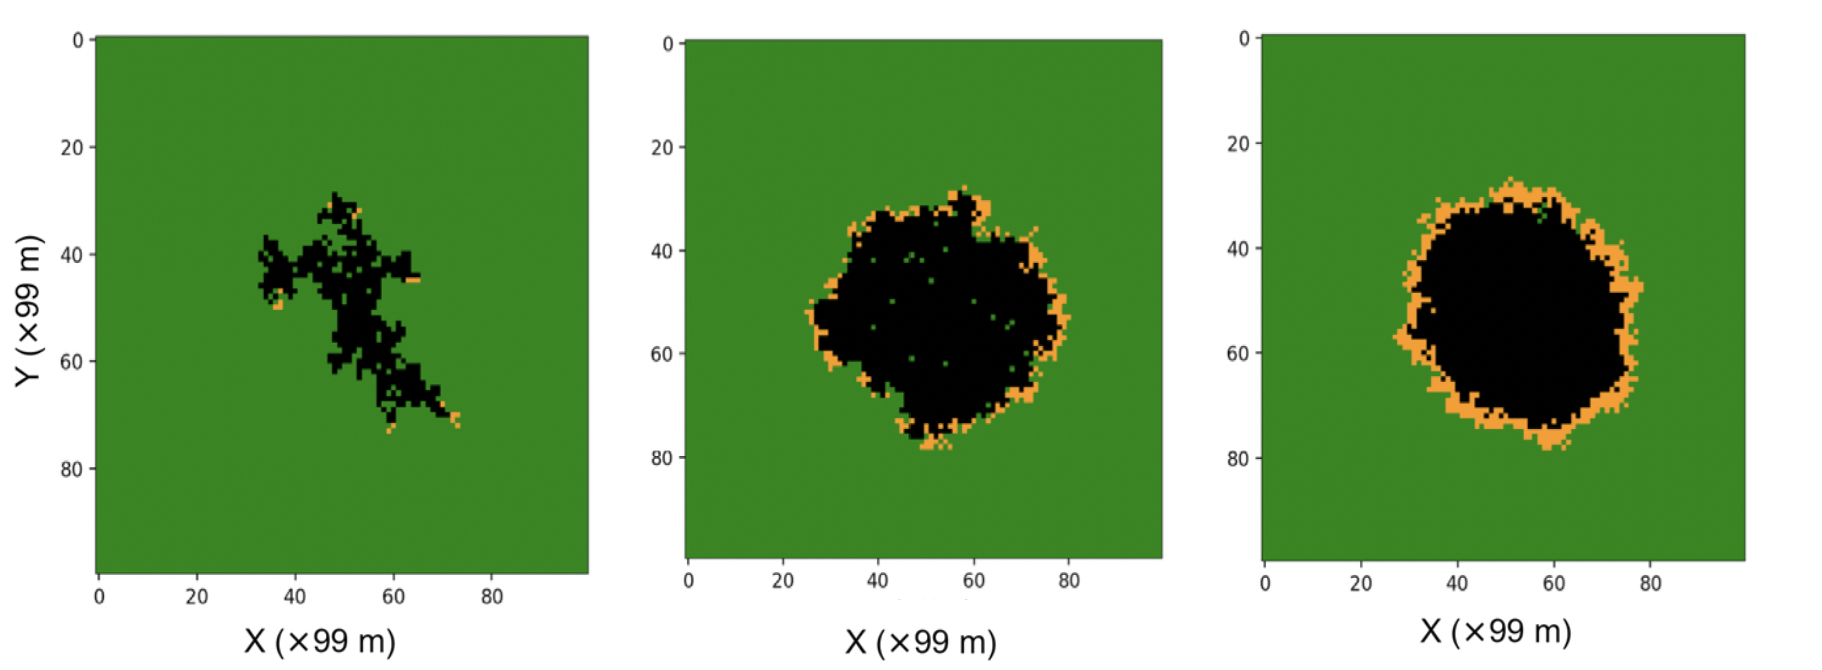
\includegraphics[width=\textwidth]{Figures/abba.png}
\caption{Left: Automaton with $\Delta t = 1$ after $N=50$ steps. Middle: Automaton with $\Delta t = 3$ after $N=50$ steps. Right: Automaton with $\Delta t = 5$ after $N=50$ steps. Colour code: \newline green = fuel cells, orange = fire cells, black = burnt cells.}
\label{f41}
\end{figure}
\newpage

\noindent We observe that with $\Delta t=1$ the fire behaviour is very sporadic and unpredictable. To obtain a measure of uncertainty in the evolution of the system, each simulation is repeated $5$ times. Across the different runs, the fire moves in random directions and does not have any overall net movement in a particular direction. \newline \indent For $\Delta t=2$, the final percentage of burnt cells after the simulation is equal to $14.36\pm2\%$, resulting in a fire spreading rate of 14.36 cells per $N$. With $\Delta t=3$ we observe that the spread of fire is more radially uniform, and for $\Delta t=5$ the fire front is thicker as there are more fire cells present. For $\Delta t=3$ the final percentage of burnt cells is equal to $38.86\pm2\%$, giving a rate of fire spread of 38.86 cells per $N$. Similarly, running the simulation for $\Delta t=5$ gives us a final percentage of burnt cells equal to $50.36\pm2\%$, corresponding to a rate of spread of $50.36$ cells per $N$. We observe that increasing $\Delta t$ from 2 to 5 results in the rate of fire spread increasing by a factor of $3.51\pm0.05$. \newline \indent The implication of these results is that the fire duration $\Delta t$ is a critically important factor when estimating the rate of spread. Applying this to real fires, our result suggests that the longer a fire is burning in one particular area, the greater the total rate of fire spread will be.\newline \indent To analyse the distribution of the percentage of burnt cells, we find the average occurrence of each value of percentage burnt. We create a simulation with a $25\times25$ grid of fuel cells and start the fire as a $5\times5$ square in the centre of the grid. The simulation is run for $N=50$ steps and we use values of $\Delta t=1,2,3$. Figures \ref{f42} and \ref{f43} show the distribution of the final percentage of burnt cells across $1000$ runs of the simulation for $\Delta t=1$ and $\Delta t=3$ respectively.

\begin{figure}[H]
\begin{center}
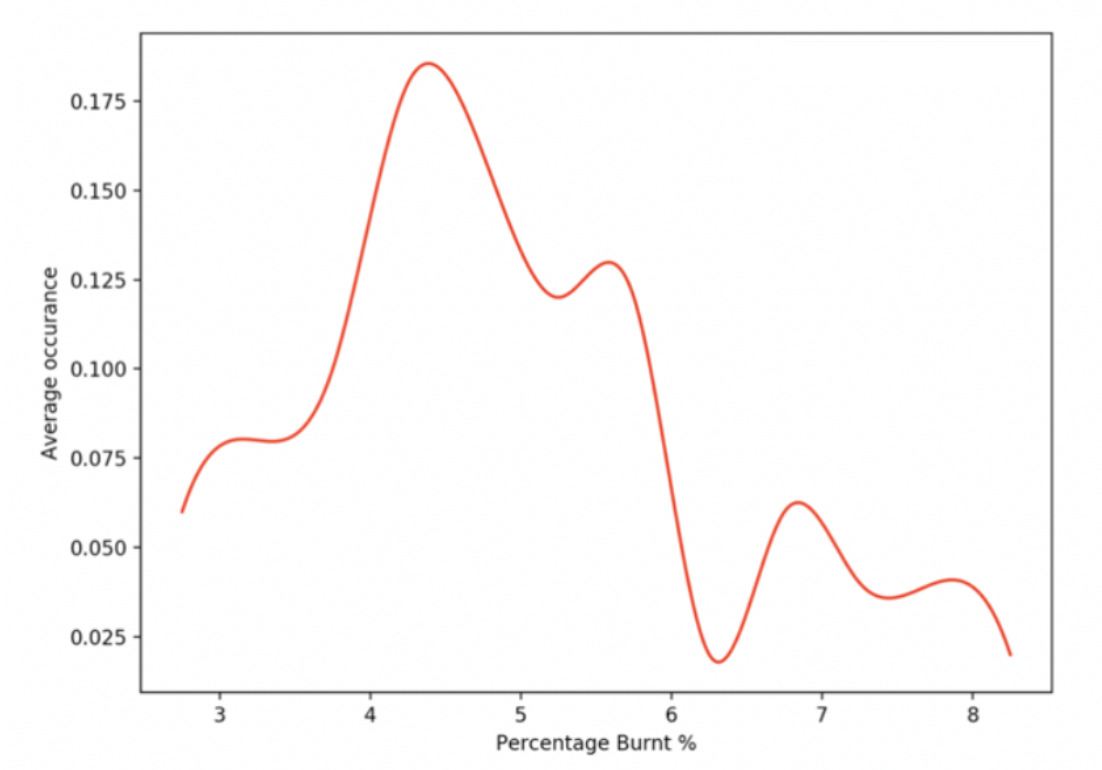
\includegraphics[width=0.9\textwidth]{Figures/ffff1.png}
\caption{Average occurrence of the percentage of burnt cells across 1000 simulations. Grid size: $(25\times 25)$ fuel cells, fire duration $\Delta t=1$, simulation duration $N=50$ time steps.} 
\label{f42}
\end{center}
\end{figure}

\begin{figure}[H]
\begin{center}
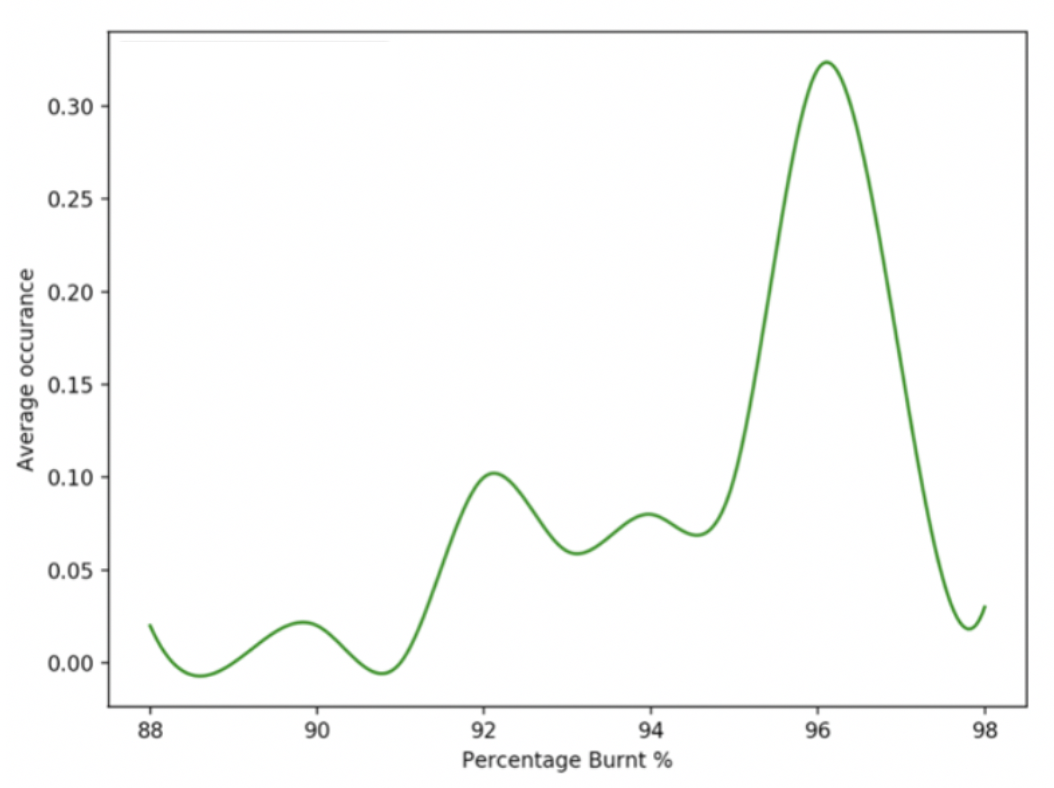
\includegraphics[width=0.9\textwidth]{Figures/ffff2.png}
\caption{Average occurrence of the percentage of burnt cells across 1000 simulations. Grid size: $(25\times 25)$ fuel cells, fire duration $\Delta t=3$, simulation duration $N=50$ time steps} 
\label{f43}
\end{center}
\end{figure}

\noindent We observe from Figures \ref{f42} and \ref{f43} that the distribution of the percentage of burnt cells for both $\Delta t=1$ and $\Delta t=3$ exhibit sporadic behaviour within the range shown. However, both distributions have a distinct peak. For $\Delta t=1$ the peak occurs at $4.25\pm0.3\%$ whilst for $\Delta t=3$ the peak occurs at $96.0\pm0.1\%$. \newline \indent The difference in these distributions shows a dramatic increasing effect that increasing the value of $\Delta t$ has on the surface area burnt by the fires. For the values $\Delta t=1,3$, the percentage of burnt cells has a narrow peak with a $\pm 2\%$ standard deviation. With $\Delta t=1$ the probability of the percentage of burnt cells being over 10\% is effectively zero, but with $\Delta t=3$ the probability of the percentage of burnt cells being under 85\% is also nearly zero. \newline \indent Interestingly, for $\Delta t=2$ the distribution of results has no distinct trends and the spread of values resembles a sinusoidal wave. For this fire duration, the values of the percentage of burnt cells range from 5\% to 80\% with no distinct peaks in the distribution. This suggests that for a fire duration of $\Delta t = 2$, the fires propagate randomly across the landscape without a uniform fire front. \newline \indent As a model of real wildfires, our simulation suggests that fire duration is a critical parameter determining the global spread of the fires across their environment. For our model to accurately represent wildfires, the precise value of $\Delta t$ needs to be determined by comparing our simulated results to real-world fires, and matching their rate of spread.

\subsection{Effects of Elevation}\label{4.2}

To analyse the effects of elevation, we investigate how the value of the strength parameter $\alpha$ affects the fire percentage of burnt cells. We create a simulation with the addition of an elevation parameter, represented by a height function $h=h(x,y)$ where $x$ and $y$ are the coordinates of each cell. Our test simulation consists of a 100$\times$100 grid of fuel cells, with 5$\times$5 fire cells at its centre, burning for a fire duration of $\Delta t = 3$. For this simulation, wind and embers are omitted, and we vary the value of $\alpha$ from $0.1$ to $0.5$ in steps of $0.1$. The elevation function used is $h(x,y)= x+y$, providing a uniform gradient. Figure \ref{f44} shows the evolution of the percentage of burnt cells in the array over time for each value of $\alpha$, for a duration of $N=100$ time steps.

\begin{figure}[H]
\begin{center}
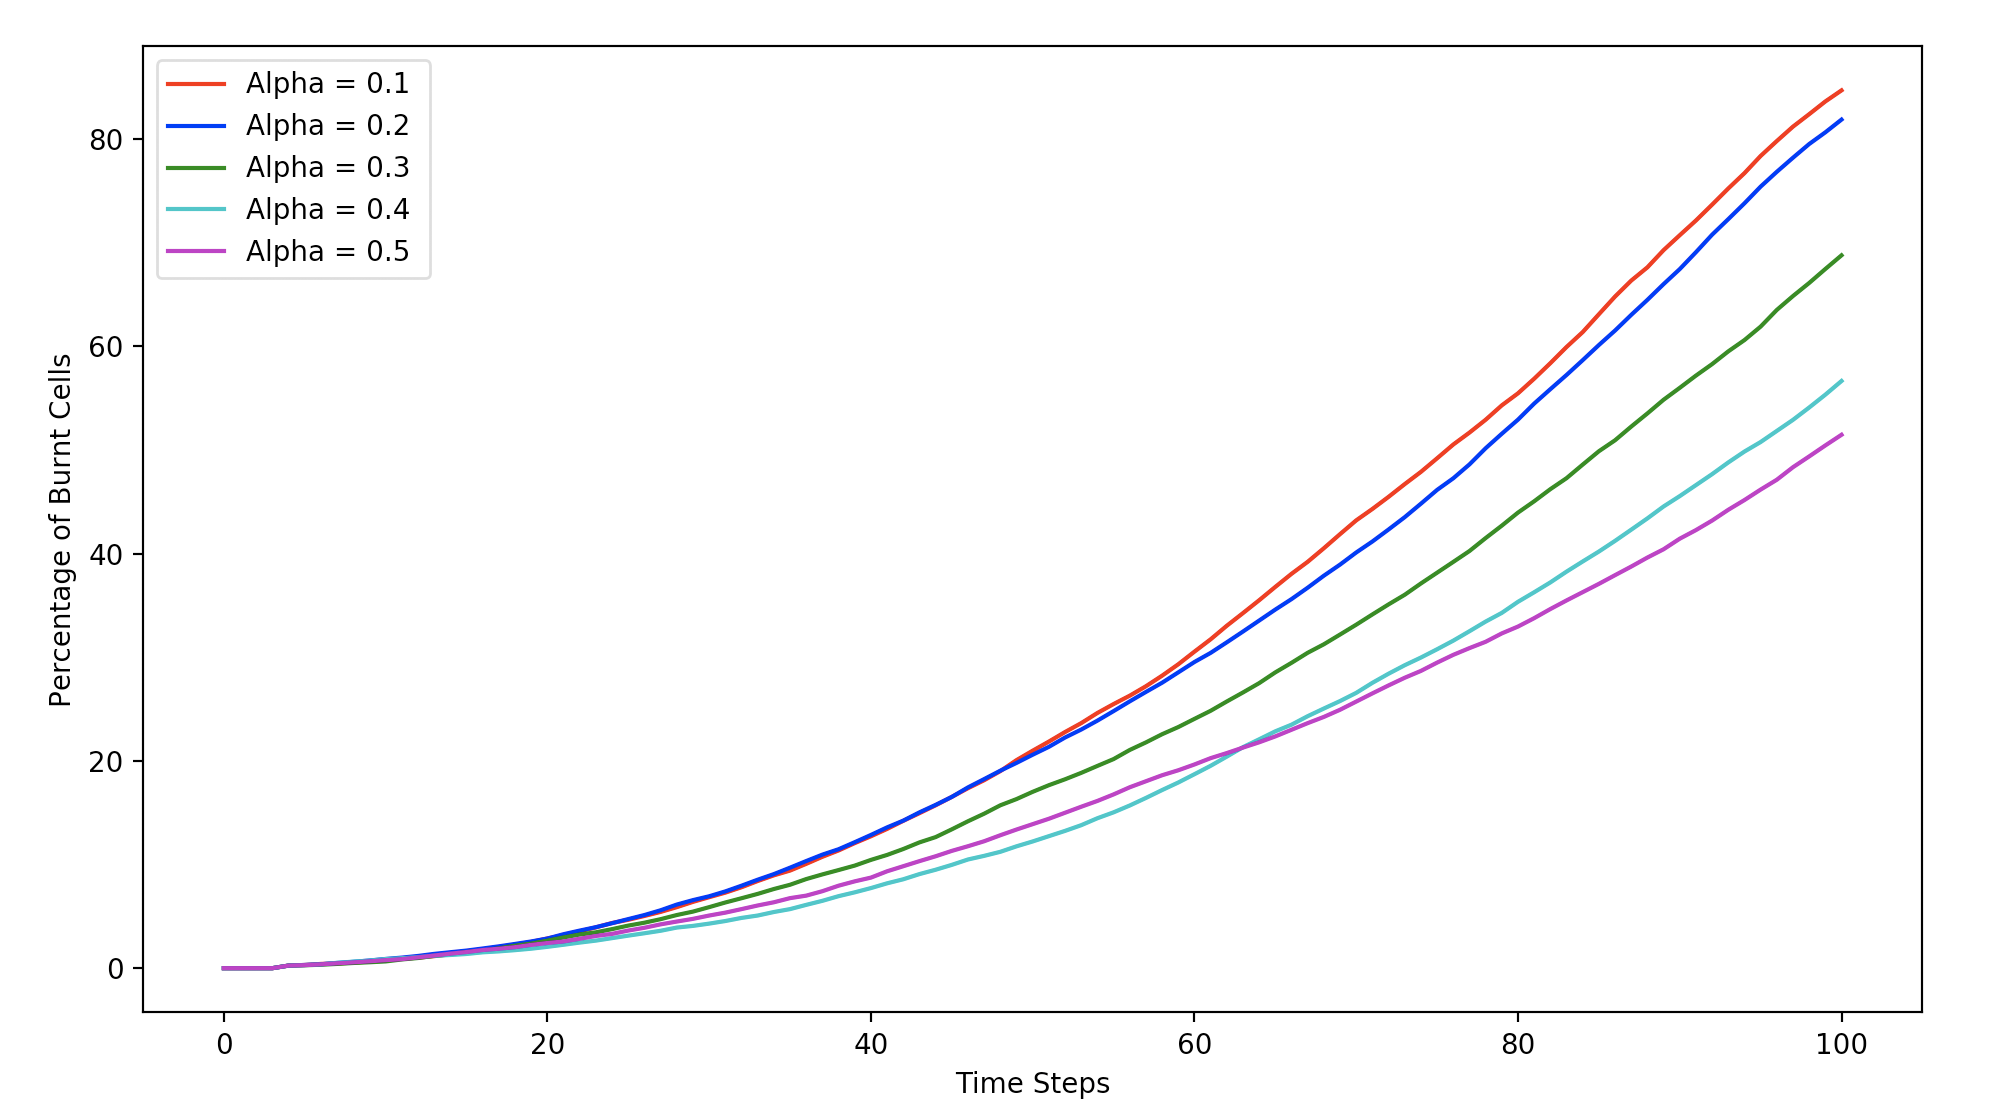
\includegraphics[width=0.9\textwidth]{Figures/f3.png}
\caption{Percentage of burnt cells for every time step $N$ with different values of $\alpha$. Initial conditions: $(5\times5)$ fire cells in the centre of a $(100\times 100)$ grid of fuel cells.} 
\label{f44}
\end{center}
\end{figure}

\noindent We observe that as $N$ increases, the number of burnt cells increases monotonically. A greater value of $\alpha$ results in a lesser rate of spread for the simulated fire. For example, when $\alpha=0.1$ the rate of spread is equal to $87.65\pm0.2$ cells per $N$ whilst for $\alpha=0.5$ the rate of spread is equal to $49.03\pm0.2$ cells per $N$. By increasing the value of $\alpha$ from 0.1 to 0.5 the rate of fire spread changes by a factor $1.788\pm0.04$. This result implies that the effect of elevation reduces the overall rate of fire spread. Physically, the simulation suggests that fire is restricted by the effects of elevation, particularly large differences in elevation. We find the specific value of $\alpha$ that completely prevents fire from spreading downhill, by using the same simulation discussed in Section \ref{4.2}. We continue increasing the value of $\alpha$ until we find that the fire doesn't spread downhill at all, and obtain a result of $\alpha=1.2\pm0.05$. Physically, this implies that there is a point in the simulation when the effects of elevation are so strong that a fire would not be able to spread downhill at all.

\subsection{Effects of Wind}\label{4.3}

To find how the wind parameter affects the fire spread, we create a simulation where the effect of changing the value of $\beta$ can be seen. This simulation consists of a column of fuel cells with a width of 40 cells and height of 100 cells. We start 5$\times$5 fire cells in the centre of one end of the column so the fire can only travel down the column. The wind vector is chosen as $\mathbf{w}=(0,5)$ so the wind is directed up the column of cells. We run this simulation with values of $\beta$ ranging from 0.1 to 0.5 in steps of 0.1. Figure \ref{f45} shows how the percentage of burnt cells evolves in time for each value of $\beta$ used.

\begin{figure}[H]
\begin{center}
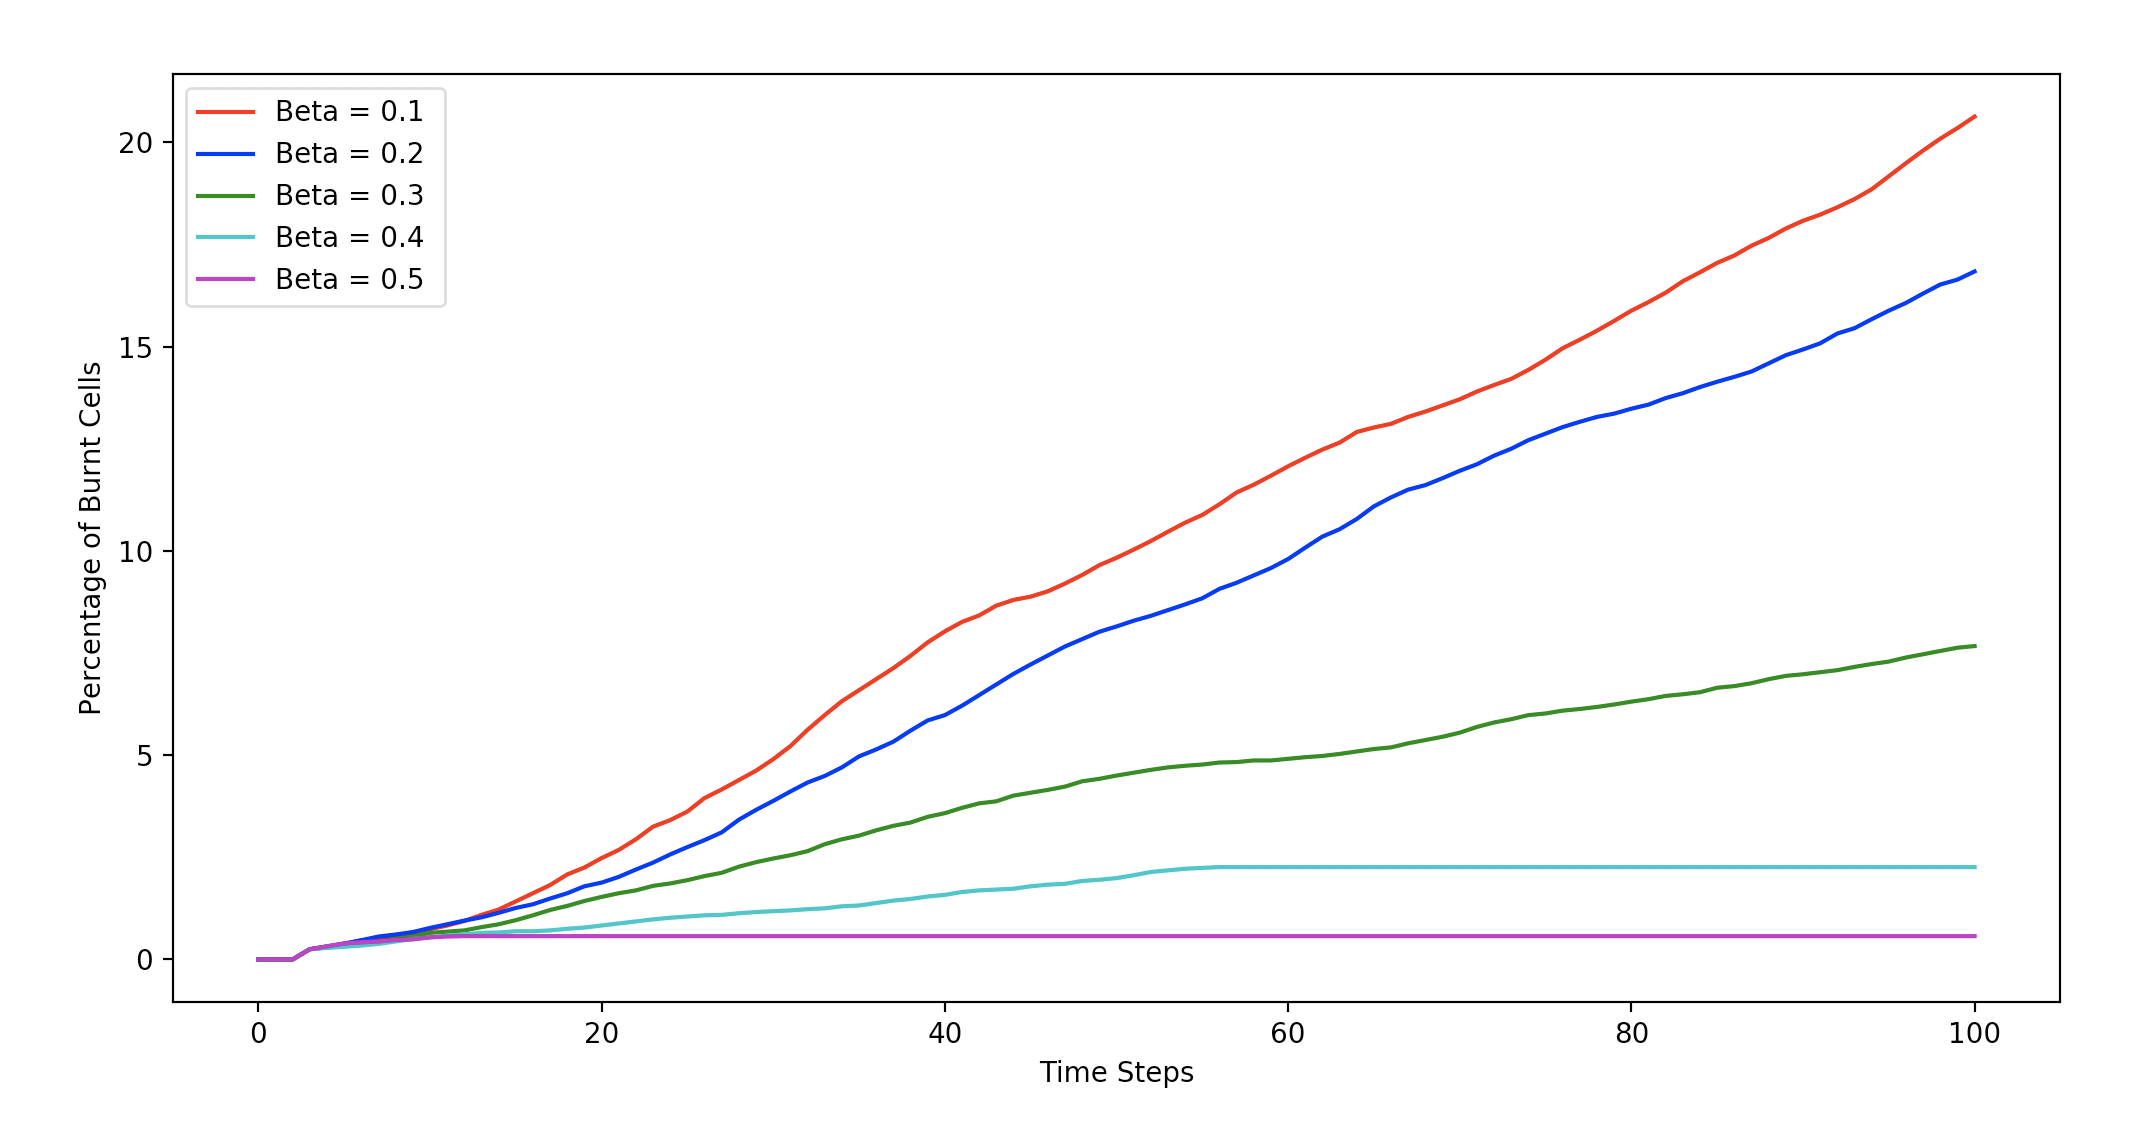
\includegraphics[width=0.9\textwidth]{Figures/f4.png}\caption{The values of percentage of burnt cells for every $N$ for different values of $\beta$} 
\label{f45}
\end{center}
\end{figure}

\noindent We observe that for a greater value of $\beta$, the percentage of burnt cells for the same $N$ is smaller. For $\beta=0.5$ we see that the fire burns out relatively quickly, extinguishing in $N \approx 10$ time steps, but for $\beta=0.1$ the percentage of burnt cells is still increasing at $N=100$. At $N=100$ and $\beta=0.5$ the percentage of burnt cells is equal to $0.57\pm0.1\%$ whereas for $\beta=0.1$ this value is equal to $20.14\pm2\%$. \newline \indent These results imply that wind blowing in the opposite direction to fire spread has a negative impact on the rate of fire spread. Physically this suggests that the danger of fire spread is considerably decreased if the wind is blowing in the opposite direction. It should be noted that the parameter $\beta$ needs to be determined via empirical analysis, comparing the effect of wind on real bushfires and our simulated results. \newline \indent To find physical limits for the parameter $\beta$, we use this simulation to find the value of $\beta$ where the fire is completely restricted by the wind. We increase the value of $\beta$ until we find that the fire does not spread at all, and observe this value to be at $\beta=0.95\pm0.05\%$. This value signals the point where the simulated strength of the wind is so great that fire travelling against the wind is effectively extinguished. To continue our analysis, we study the effect of wind blowing in the same direction as the fire spread in Section \ref{4.5}.

\subsection{Effects of Embers}\label{4.4}

Our model incorporates several parameters which relate to the introduction of embers into the system. To analyse this phenomenon we create a simulation where the number of embers $E$ released by a fire cell is varied. We create a simulation with $100\times100$ flammable cells and start $5\times5$ fire cells in its centre, with the initial parameters $\Delta t=2$, $t_f=10$, $M=5$, $\sigma=2$. The number of embers emitted from a cell are varied between the values $E=3,4,5,6,7$. Figure \ref{f46} shows how the percentage of burnt cells increases with time for each of these values. 

\begin{figure}[H]
\begin{center}
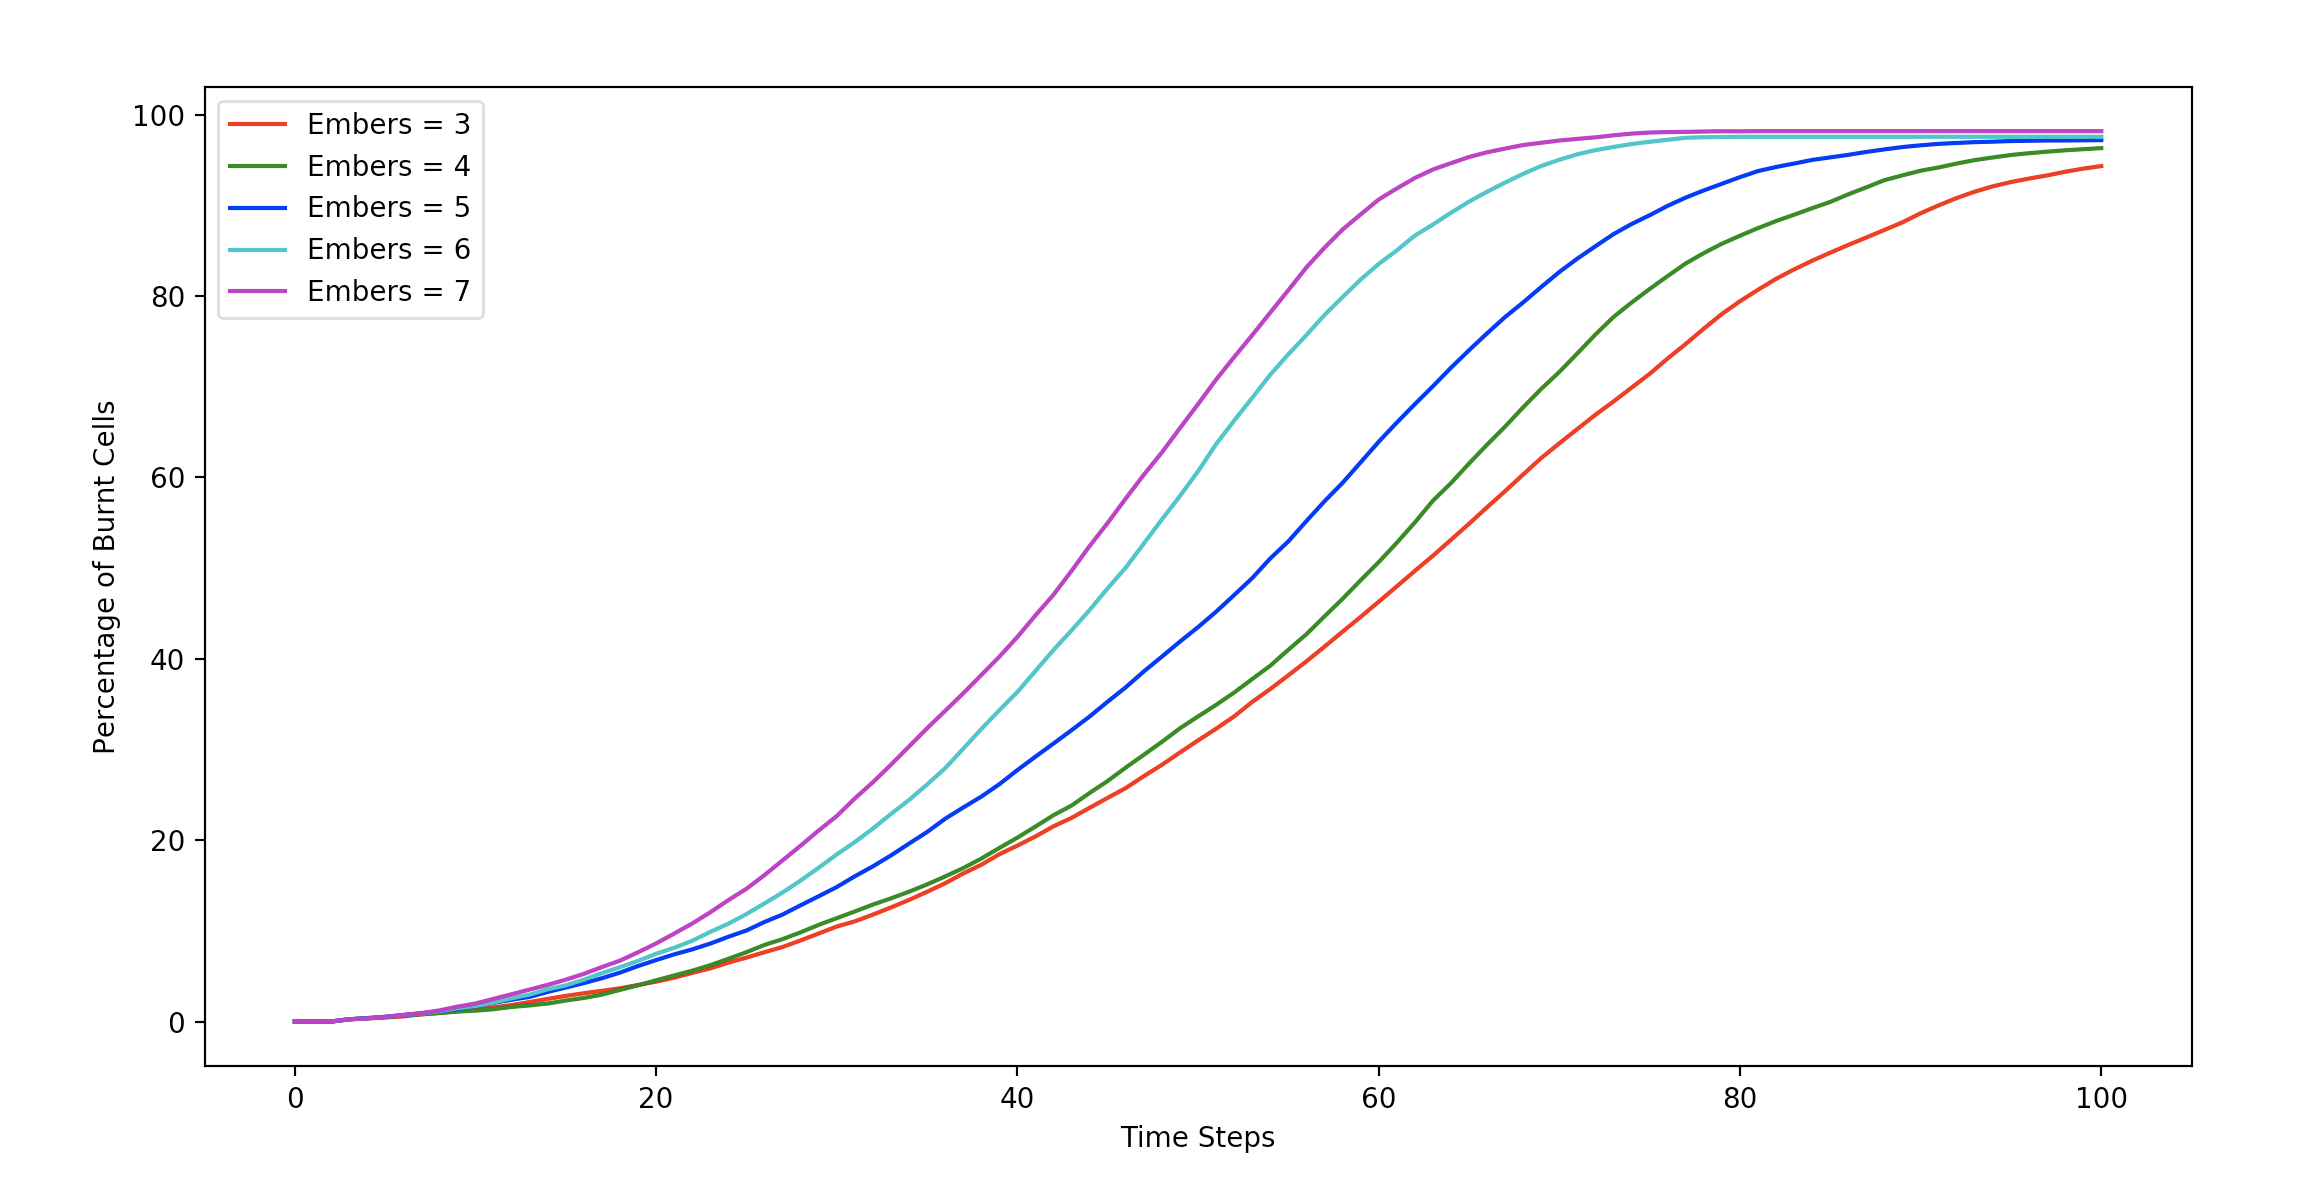
\includegraphics[width=0.9\textwidth]{Figures/f5.png}
\caption{The values of percentage of burnt cells for every N for different values of E.} 
\label{f46}
\end{center}
\end{figure}

\noindent We observe that the introduction of embers has a dramatic effect on the rate of fire spread and that a larger number of embers results in a greater percentage of burnt cells at every time step. For example, when $E=3$ the rate of fire spread is equal to $94.53\pm2$ cells per $N$. We recall from Section \ref{4.1} that without any additional environmental parameters the rate of fire spread for $\Delta t=2$ is equal to 14.36 cells per $N$. This implies that by introducing embers into the simulation the rate of fire spread increases by at least a factor of $6.583\pm2$. Using this result we infer that one of the primary methods of fire transition is through the embers emitted by a fire. Without the spreading of embers, fires would be much more contained.

\subsection{Fuel Ignition Probability}\label{4.5}

To further understand the effect which each environmental aspect of model has on the simulated fire spread, we analyse how the probability of ignition of a cell changes with the addition of different parameters and obstacles. We perform a simulation with a 50$\times$50 grid of fuel cells with 5$\times$5 initial fire cells in the top left corner. The simulation is run for N=200 steps with $\Delta t=2$. To obtain the fuel ignition probability, the average result for each cell is calculated across 1000 runs with identical initial conditions. Figure \ref{f47} shows two probability heat maps; one for this simulation with no additional parameters and one for a simulation with a $30\times30$ block of non-flammable cells in the centre of the grid.

\begin{figure}[h!]
\begin{center}
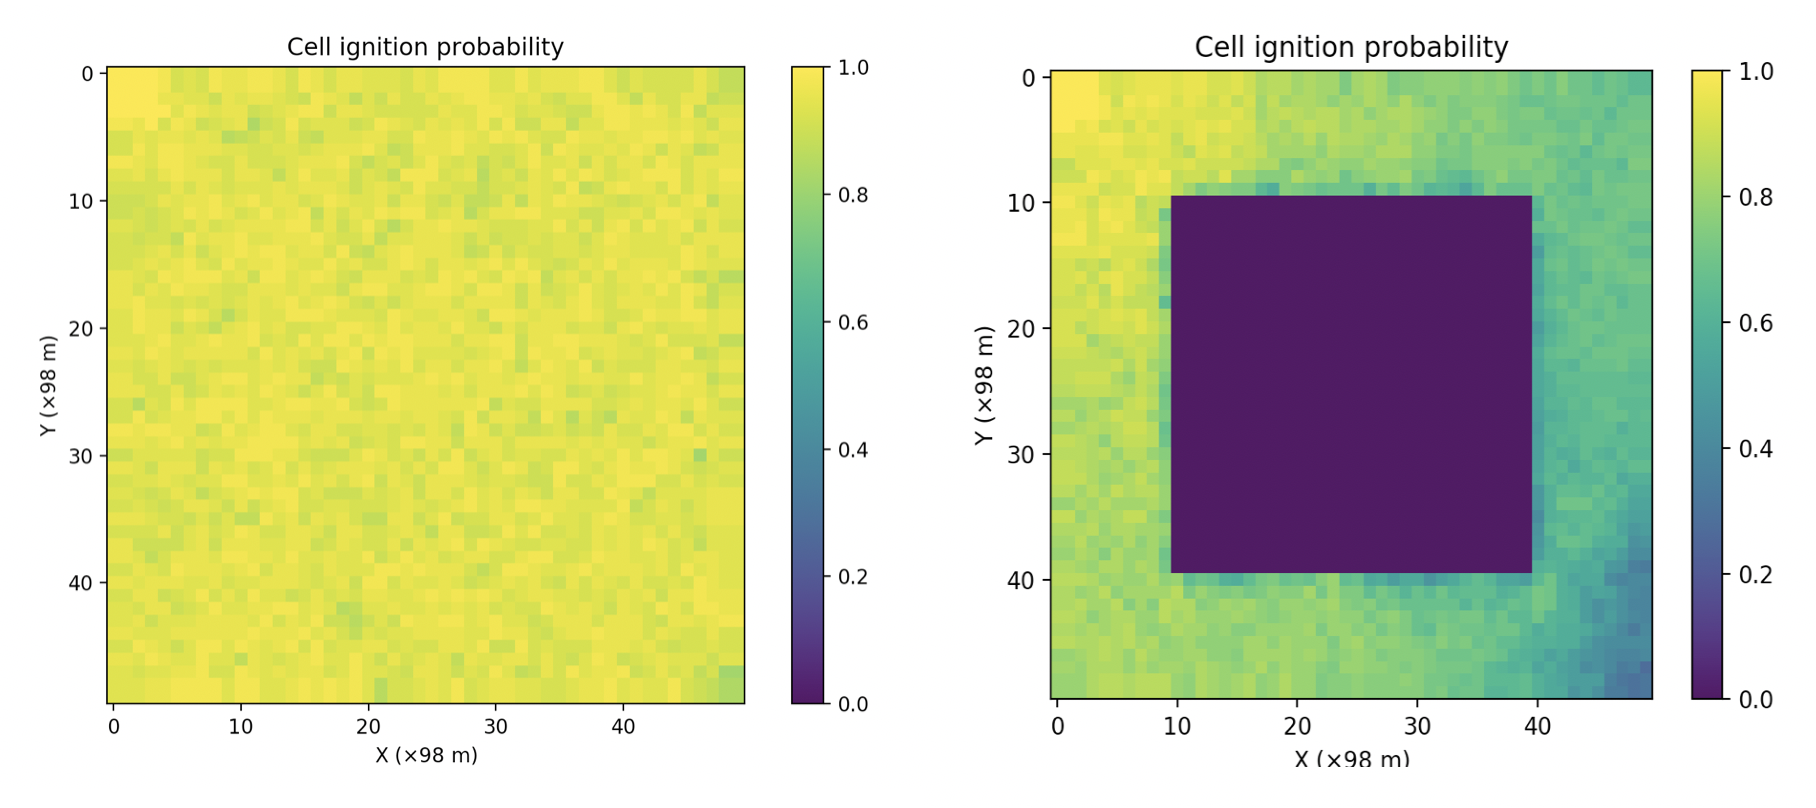
\includegraphics[width=0.8\textwidth]{Figures/h.png}
\caption{Probability heat maps of ignition. Left: result of simulation without any wind, elevation, embers or obstacles added. Right: result of identical simulation with a $30\times30$ block of non-flammable cells added at the centre.}\label{f47} \end{center}
\end{figure} 

\noindent We compare the two results by investigating the probability of ignition of the cell in the bottom right corner, located opposite to the starting fire at position $(49,49)$. In the absence of obstacles, the probability of ignition for this cell is equal to $0.84$, and in the presence of a $30 \times 30$ block of non-flammable material, this probability decreases to $0.32$. We repeat the same process with the addition of elevation, using $\alpha = 0.3$ and an elevation function $h(x,y) = 100+\sin(\frac{x}{10})+ 20\cos(\frac{y}{100})$. For these conditions, without the presence of the non-flammable cells the probability of ignition of the corner cell is $0.08$. With the block of non-flammable cells included, the probability of ignition is equal to $0.01$.\newline
\indent We repeat the procedure with the addition of wind, using a wind vector $\mathbf{w}=(5,-5)$ and $\beta=0.3$. The probability of ignition with these conditions, without the block of non-flammable cells is equal to $0.99$, and the probability of ignition with the block is $0.88$. We then calculate the ignition probability of the cell at $(49,49)$ with the addition of embers, with the following conditions: $E=10$, $M=10$, $t_f=5$ and $\sigma=2$. In the scenario without the block of non-flammable cells, the probability of ignition is equal to $0.96$, whereas in the presence of the block the ignition probability is $0.92$. We observe that when the effects of embers are taken into account the probability of ignition increases by a factor of 1.14$\pm0.01$. If both elevation and embers are taken into account, then the probability of ignition decreases by a factor of  10.5$\pm0.5$. \newline \indent We concur from these results that if wind is blowing in the direction of a cell, then the probability of ignition to that cell is greater by a factor of $1.20\pm0.01$. Physically this suggests that the most dangerous place to be in relation to a fire is directly in line with the direction of the wind. Our simulation implies that to reduce the probability of a wildfire reaching a particular location, the number of nearby non-flammable obstacles should be increased. \newpage 
\subsection{Numerical Fire Equations}\label{numericalfire}
We use our fire simulation to find a set of equations that describe the probability of ignition of a particular cell. We determine the relationships between the probability of ignition $P$ and the following variables: the  number of time steps $T$ the fire has been spreading for since the fire started, the distance $X$ between a selected cell and the nearest fire cell at the start of the simulation, the value of $\beta$. We create a simulation consisting of a single fire cell with $\Delta t = 2$  at the centre of a $30\times30$ grid of fuel cells, running for $N=20$ time steps. No elevation, wind or embers are included for simplicity.  Figure \ref{f48} shows the resulting ignition probability heat map after 1000 runs.

\begin{figure}[h!]
\begin{center}
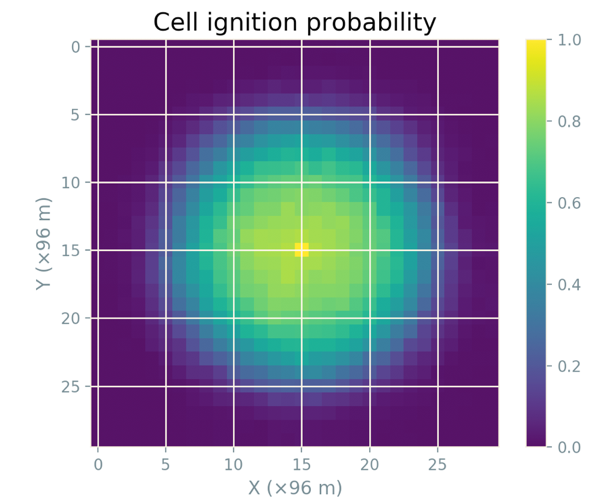
\includegraphics[scale=0.5]{Figures/h5.png}
\caption{Ignition probability heat map for a simulation with a single initial fire cell in the middle of $30\times30$ fuel cells, after $N=20$ steps.} 
\label{f48}
\end{center}
\end{figure} 

\noindent We observe that the probability of ignition $P$ of a given cell decreases with distance from the starting fire, following an approximate power law. The exact relationship is determined in conjunction with the dependence of $P$ on the number of time steps $N$ for which the simulation is run for. We run the same simulation used to create Figure \ref{f48} while varying the number of steps $T$ the simulation is run for. To obtain numerical values in this relationship, we generate a large number of identical simulations and obtain power law fittings between $P$ and the parameters $X,T$ and $\beta$. The resulting equation combines all of these parameters, giving us a function $P(T,X,\beta)$:

\begin{equation}
    \large
    P(T,X,\beta) = \begin{cases}\chi_1 \frac{T^{2.049} \beta^{1.598}}{X^{0.2017}} + \chi_2 \pm 0.1464& \mbox{\normalsize when wind blows toward the cell}\\
    \chi_3 \frac{T^{2.049}} {X^{0.2017} \beta^{2.243}} + \chi_4 + \pm 0.1964& \mbox{\normalsize when wind blows away from the cell}
    \end{cases}
    \label{p2}
\end{equation}

\noindent where the constants $\chi_1 = 5.69 \pm0.05\times 10^{-4}$, $\chi_2=0.577\pm 0.05$,$\chi_3=8.04\pm0.2\times 10^{-8},$ and $\chi_4=0.212\pm0.05$. Equation \ref{p2} can be used to estimate the probability of ignition for a simulation of size $30 \times 30$ grid with a single fire cell of $\Delta t=2$ at the centre of the grid, assuming the following conditions are satisfied: $T>20$ and $0.05<\beta<0.1$. \newline 
\indent We find that for a very large value of $T$ or a very low value of $X$ the probability of ignition is very close to 1. This implies that in such conditions it is effectively guaranteed that the fire will ignite a particular cell. Moreover, we can see that the relationship between the probability of ignition and the strength of wind is very dependent on the direction of the wind. In terms of real wildfires, we postulate that the areas with the lowest chances of ignition need to be far away from the fire and in a direction where the wind is blowing away from the fire.

\subsection{Limits of the Fire Model}\label{modellimits}

We have observed how our model replicates wildfire behaviour with the effects of different environmental parameters. We demonstrate that elevation, wind and spotting can all be incorporated into the cellular automaton simulation with physically sound results, showing that our methodology is a valid starting point for a wildfire simulation. \newline \indent The central limitation of our model is in determining the exact values of the fire parameter $\Delta t$ and environmental strength parameters $\alpha, \beta, E,M,t_f$ and $\sigma$. We observe a dramatic change in fire behaviour depending on the value of $\Delta t$, where the difference between $\Delta t=1$ and $\Delta t=3$ changes the eventual area burnt by fire by $80\%$. To model fire in a particular situation, we require knowledge of which value of $\Delta t$ is physically accurate. Obtaining this information requires a large amount of precise historical data and may prove challenging. Likewise, without knowing appropriate values of $\alpha$ and $\beta$ the model cannot be expected to accurately reproduce real fire behaviour. \newline \indent Furthermore, the environmental parameters within our model do not always yield physical results. For example, if we set $\alpha>4.0$ or $\beta>4.0$ in a simulation, then the fire model shows all fire being instantly extinguished, with no spread in any direction. Another non-physical result can be obtained by configuring the ember parameters $E,M,t_f$ and $\sigma$. There exists a critical point where the effects of embers become so large that the fire behaviour becomes explosive and extremely non-physical, spreading across the map with increasing speed until all fuel has been burned. This explosive behaviour causes the rate of fire spread to reach values of over 500 cells per $N$, depending on the values of the ember variables used. When $t_f=10$ and $\sigma=2$, the critical point occurs at $E=3M$.\newline \indent As an additional remark, the rules used within this automaton are probabilistic and do not consider the complex physics behind fire transitions. Hence there is no guarantee that these rules will realistically model fire or preserve quantities that have associated conservation laws such as energy or momentum. To obtain a picture of the true physical accuracy of our model, we compare data produced by the cellular automaton model with data from real bushfires. This is the subject of Section \ref{results_2}.